\documentclass[handout]{beamer}
%\documentclass{beamer}
\usepackage{tikz}
\def\checkmark{\tikz\fill[scale=0.4](0,.35) -- (.25,0) -- (1,.7) -- (.25,.15) -- cycle;} 
\usepackage{pifont}
\newcommand{\xmark}{\ding{55}}
\usepackage{tikz}
\usepackage{biblatex}
\usetheme{PaloAlto}
\title{An introduction to statistical inference}
\author[Ben Lambert]{Ben Lambert\inst{1}\\ \texttt{ben.c.lambert@gmail.com}}

\usepackage{datetime}
\newdate{date}{6}{7}{2021}
\date{\displaydate{date}}
\institute[University of Oxford]{
\inst{1}University of Oxford}
\beamertemplatenavigationsymbolsempty
\setbeamertemplate{sidebar left}{}
\usepackage{caption}
\usepackage{amsmath}
\usepackage{soul,xcolor}
\usepackage{multimedia}
\usepackage{bbm}
\usepackage{animate}
\usepackage{graphics}
\usepackage{graphicx}
\usepackage[makeroom]{cancel}
\usepackage{xcolor,cancel}
\captionsetup{font=footnotesize}
\usepackage[utf8]{inputenc}
\makeatletter
\newcommand\mathcircled[1]{%
  \mathpalette\@mathcircled{#1}%
}
\newcommand\@mathcircled[2]{%
  \tikz[baseline=(math.base)] \node[draw,circle,inner sep=1pt] (math) {$\m@th#1#2$};%
}
\makeatother
\definecolor{beige}{RGB}{238,213,173}

\newcommand\hcancel[2][black]{\setbox0=\hbox{$#2$}%
	\rlap{\raisebox{.45\ht0}{\textcolor{#1}{\rule{\wd0}{1pt}}}}#2} 

\bibliography{Bayes}

\begin{document}

\begin{frame}
\titlepage
\end{frame}

\begin{frame}
	\frametitle{Course plan}
	\begin{itemize}
		\item 9.30am-10.15am: lecture, ``An introduction to statistical inference''
		\item 10.45am-1pm: practical
	\end{itemize}
	
\end{frame}

\begin{frame}
	\frametitle{Outline}
	\tableofcontents
\end{frame}

\section{Science and statistics}
\frame{\tableofcontents[currentsection]}

\begin{frame}
	\frametitle{What is the aim of scientific inquiry?}
	Understand how the universe works.
	
		\begin{figure}[ht]
			\centerline{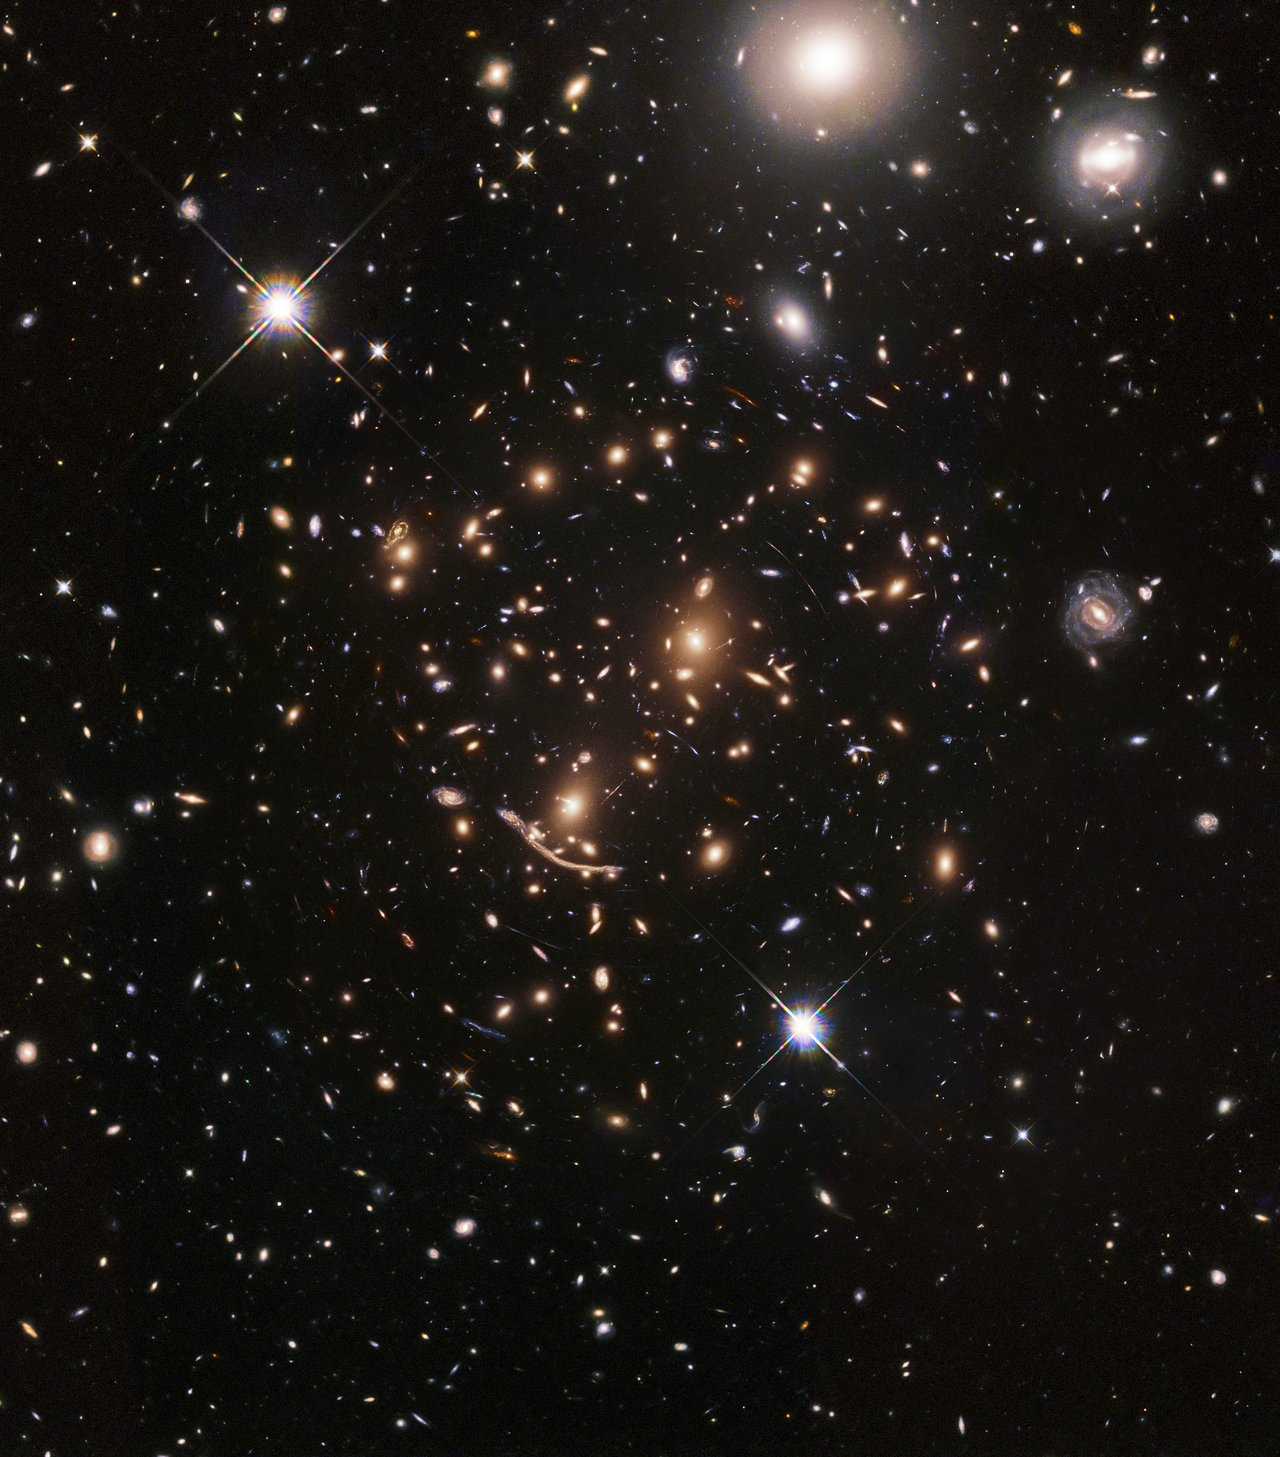
\includegraphics[width=0.6\textwidth]{./figures/universe.jpeg}}
		\end{figure}
	
\end{frame}

\begin{frame}
	\frametitle{What does it mean to understand the universe?}
	
	Understand causality.
	
\end{frame}

\begin{frame}
	\frametitle{How do we test our understanding?}
	
	Make predictions. Compare reality with our predictions.

\end{frame}

\begin{frame}
	\frametitle{What can statistical inference help with?}
	
	\begin{itemize}
		\item Generating understanding from data
		\item Testing our scientific hypotheses versus data
	\end{itemize}
	
\end{frame}

\begin{frame}
	\frametitle{But why do we need statistics?}
	
	\begin{itemize}
		\item The universe is complex
		\item Its mechanisms are not directly observable
		\item Our data contain information both about the mechanisms and other nuisance factors
	\end{itemize}
	
	Statistics provides a way to separate the signal of the mechanisms from the noise.
	
\end{frame}

\begin{frame}
	\frametitle{How statistics separates signal from noise?}
	
	\begin{equation}
	\text{observations} = \text{signal} + \text{noise}
	\end{equation}
	
	\begin{itemize}
		\item Signal contains our interesting scientific mechanism
		\item Noise contains a bunch of things not of interest
	\end{itemize}
	
	Since we do not know or observe the exact noise processes, in statistics, it is assumed that the noise is represented as being \textit{random}.
	
	\vspace{0.5cm}
	
	But random does not mean unstructured. In statistics, making assumptions about the nature of the random process allows us to bound its influence on the observed data.
	
\end{frame}

\begin{frame}
	\frametitle{Example 1: flipping a coin}
	
	Suppose we flip a coin twice. We could obtain:
	
	\begin{itemize}
		\item Two tails
		\item One head; one tail
		\item Two heads
	\end{itemize}
	
	Why can we get different outcomes each time the coin is flipped?
	
\end{frame}

\begin{frame}
	\frametitle{Different initial conditions}
	
	Precessional frequency: $\omega_N$; Magnitude of upward velocity, $u$.\footnote{\tiny From Probability, geometry, and dynamics in the toss of a thick coin, Yong and Mahadevan (2011)}
	
	\begin{figure}[ht]
		\centerline{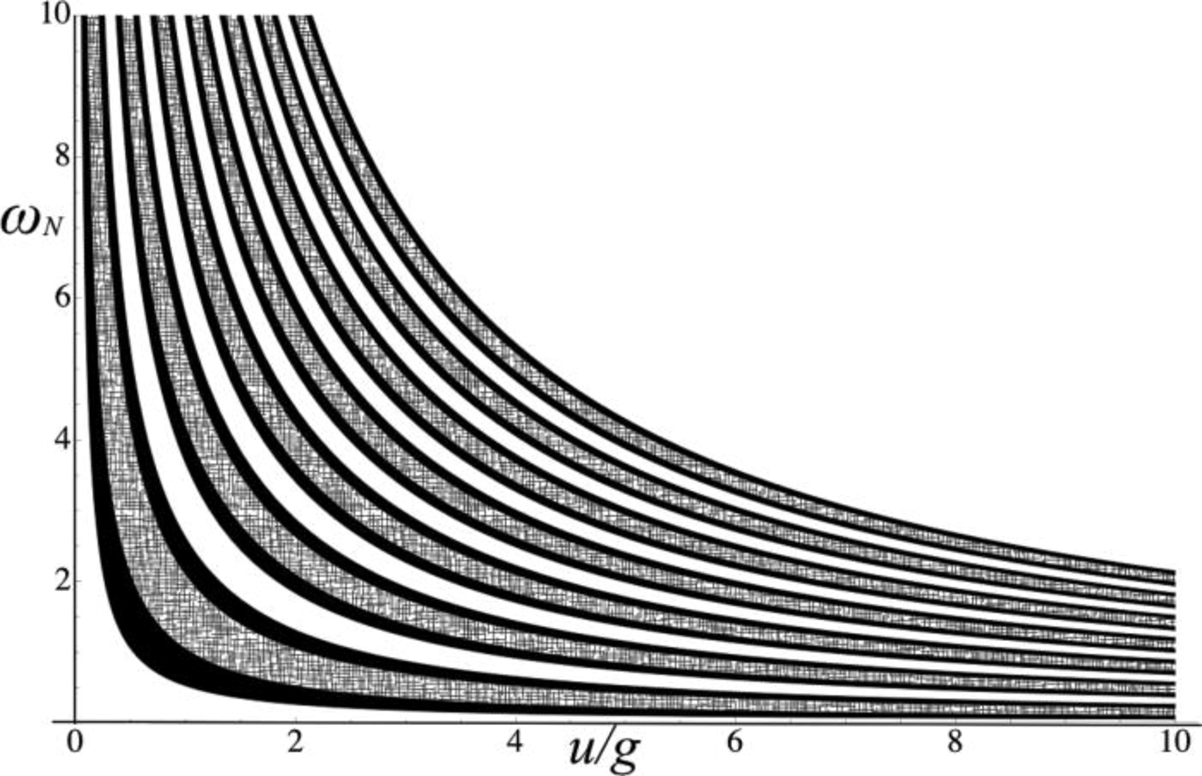
\includegraphics[width=0.6\textwidth]{./figures/coin_toss.pdf}}
	\end{figure}
	
	White indicates heads; hatched indicates lands on sides; hatched indicates tails.
	
\end{frame}

\begin{frame}
	\frametitle{Coin flip dynamics: physics approach}
	
	Solve complex equations of motion (making assumptions about flipping process). One part of the system:
	
	\begin{equation}
	\frac{d\boldsymbol{N}}{dt} = \Omega \times \boldsymbol{N}
	\end{equation}
	
	This system determines outcome given a set of initial conditions: precessional frequency and magnitude of upward velocity.
	
	\vspace{0.5cm}
	But we still don't know how different people throw a coin, so we'd need to measure this and likely represent this using randomness!
	
\end{frame}

\begin{frame}
	\frametitle{Coin flip dynamics: statistical approach}
	
	Assume outcome of a coin flip is a random variable with a probability of landing heads up (binomial distribution\footnote{If we forget the landing on side situation.}). Implicitly:
	
	\begin{figure}[ht]
		\centerline{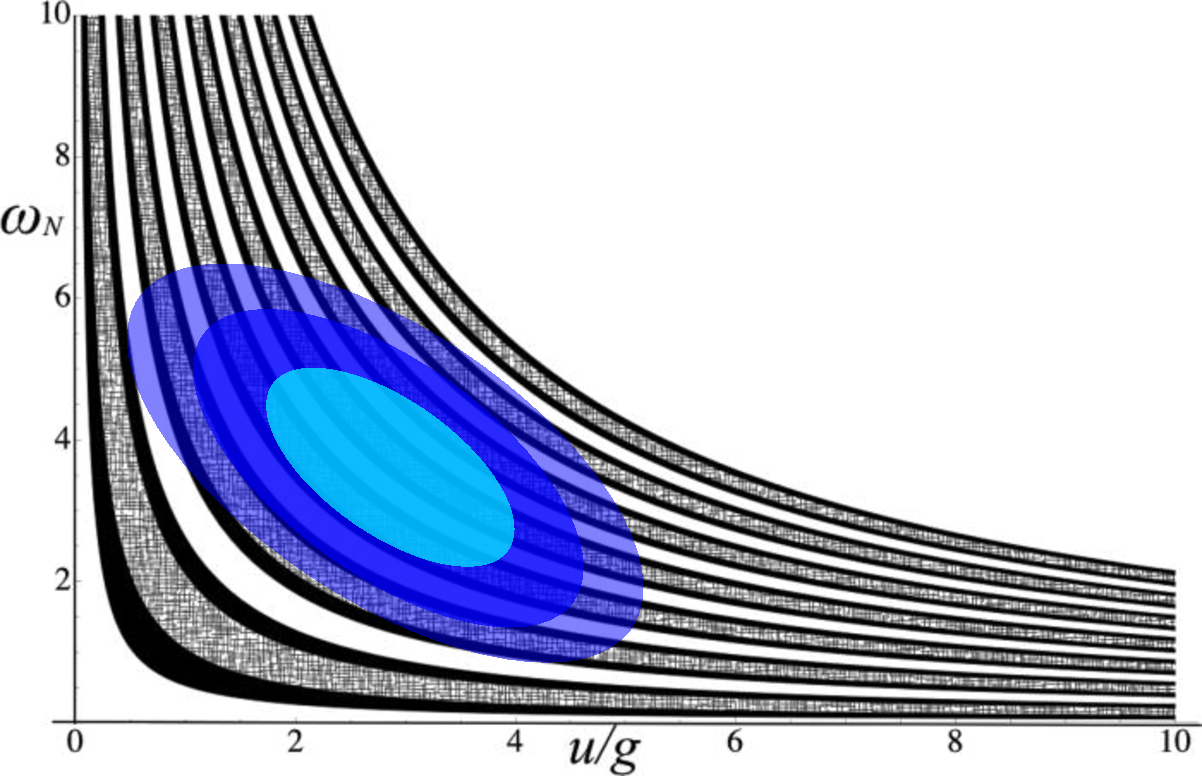
\includegraphics[width=0.6\textwidth]{./figures/coin_toss_density.pdf}}
	\end{figure}
	
\end{frame}

\begin{frame}
	\frametitle{Example 2: determining COVID-19 seropositivity}
	Imagine we want to determine the proportion of the UK population who have COVID-19 antibodies. To do this, we find 10 individuals and test their blood.
	
	\begin{figure}[ht]
		\centerline{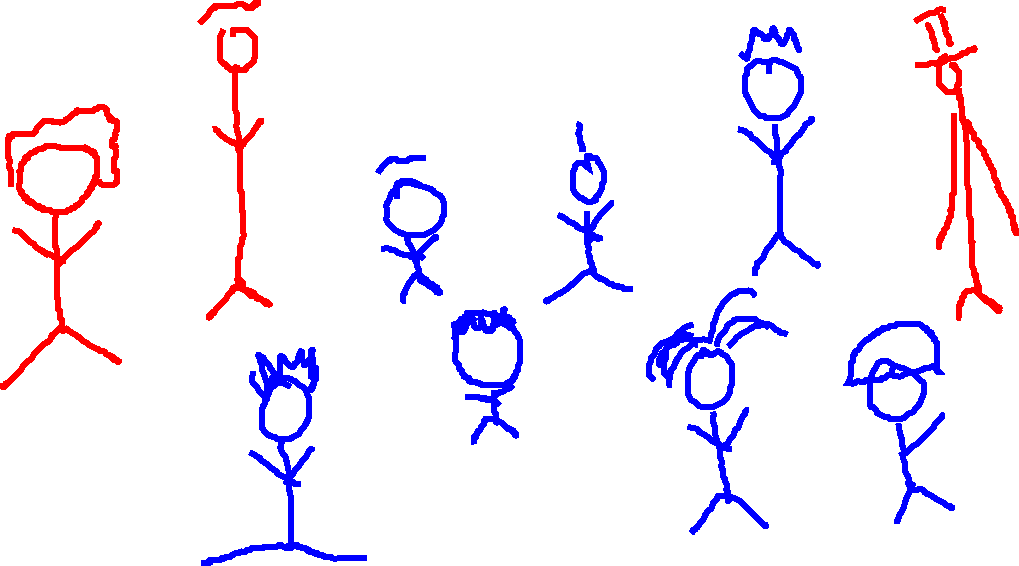
\includegraphics[width=0.6\textwidth]{./figures/covid_stick.pdf}}
	\end{figure}
	
	Does this mean $3/10=30\%$ of the UK population have these antibodies?
	
\end{frame}

\begin{frame}
	\frametitle{The sampling process yields variation in outputs}
	No.
	
	\begin{figure}[ht]
		\centerline{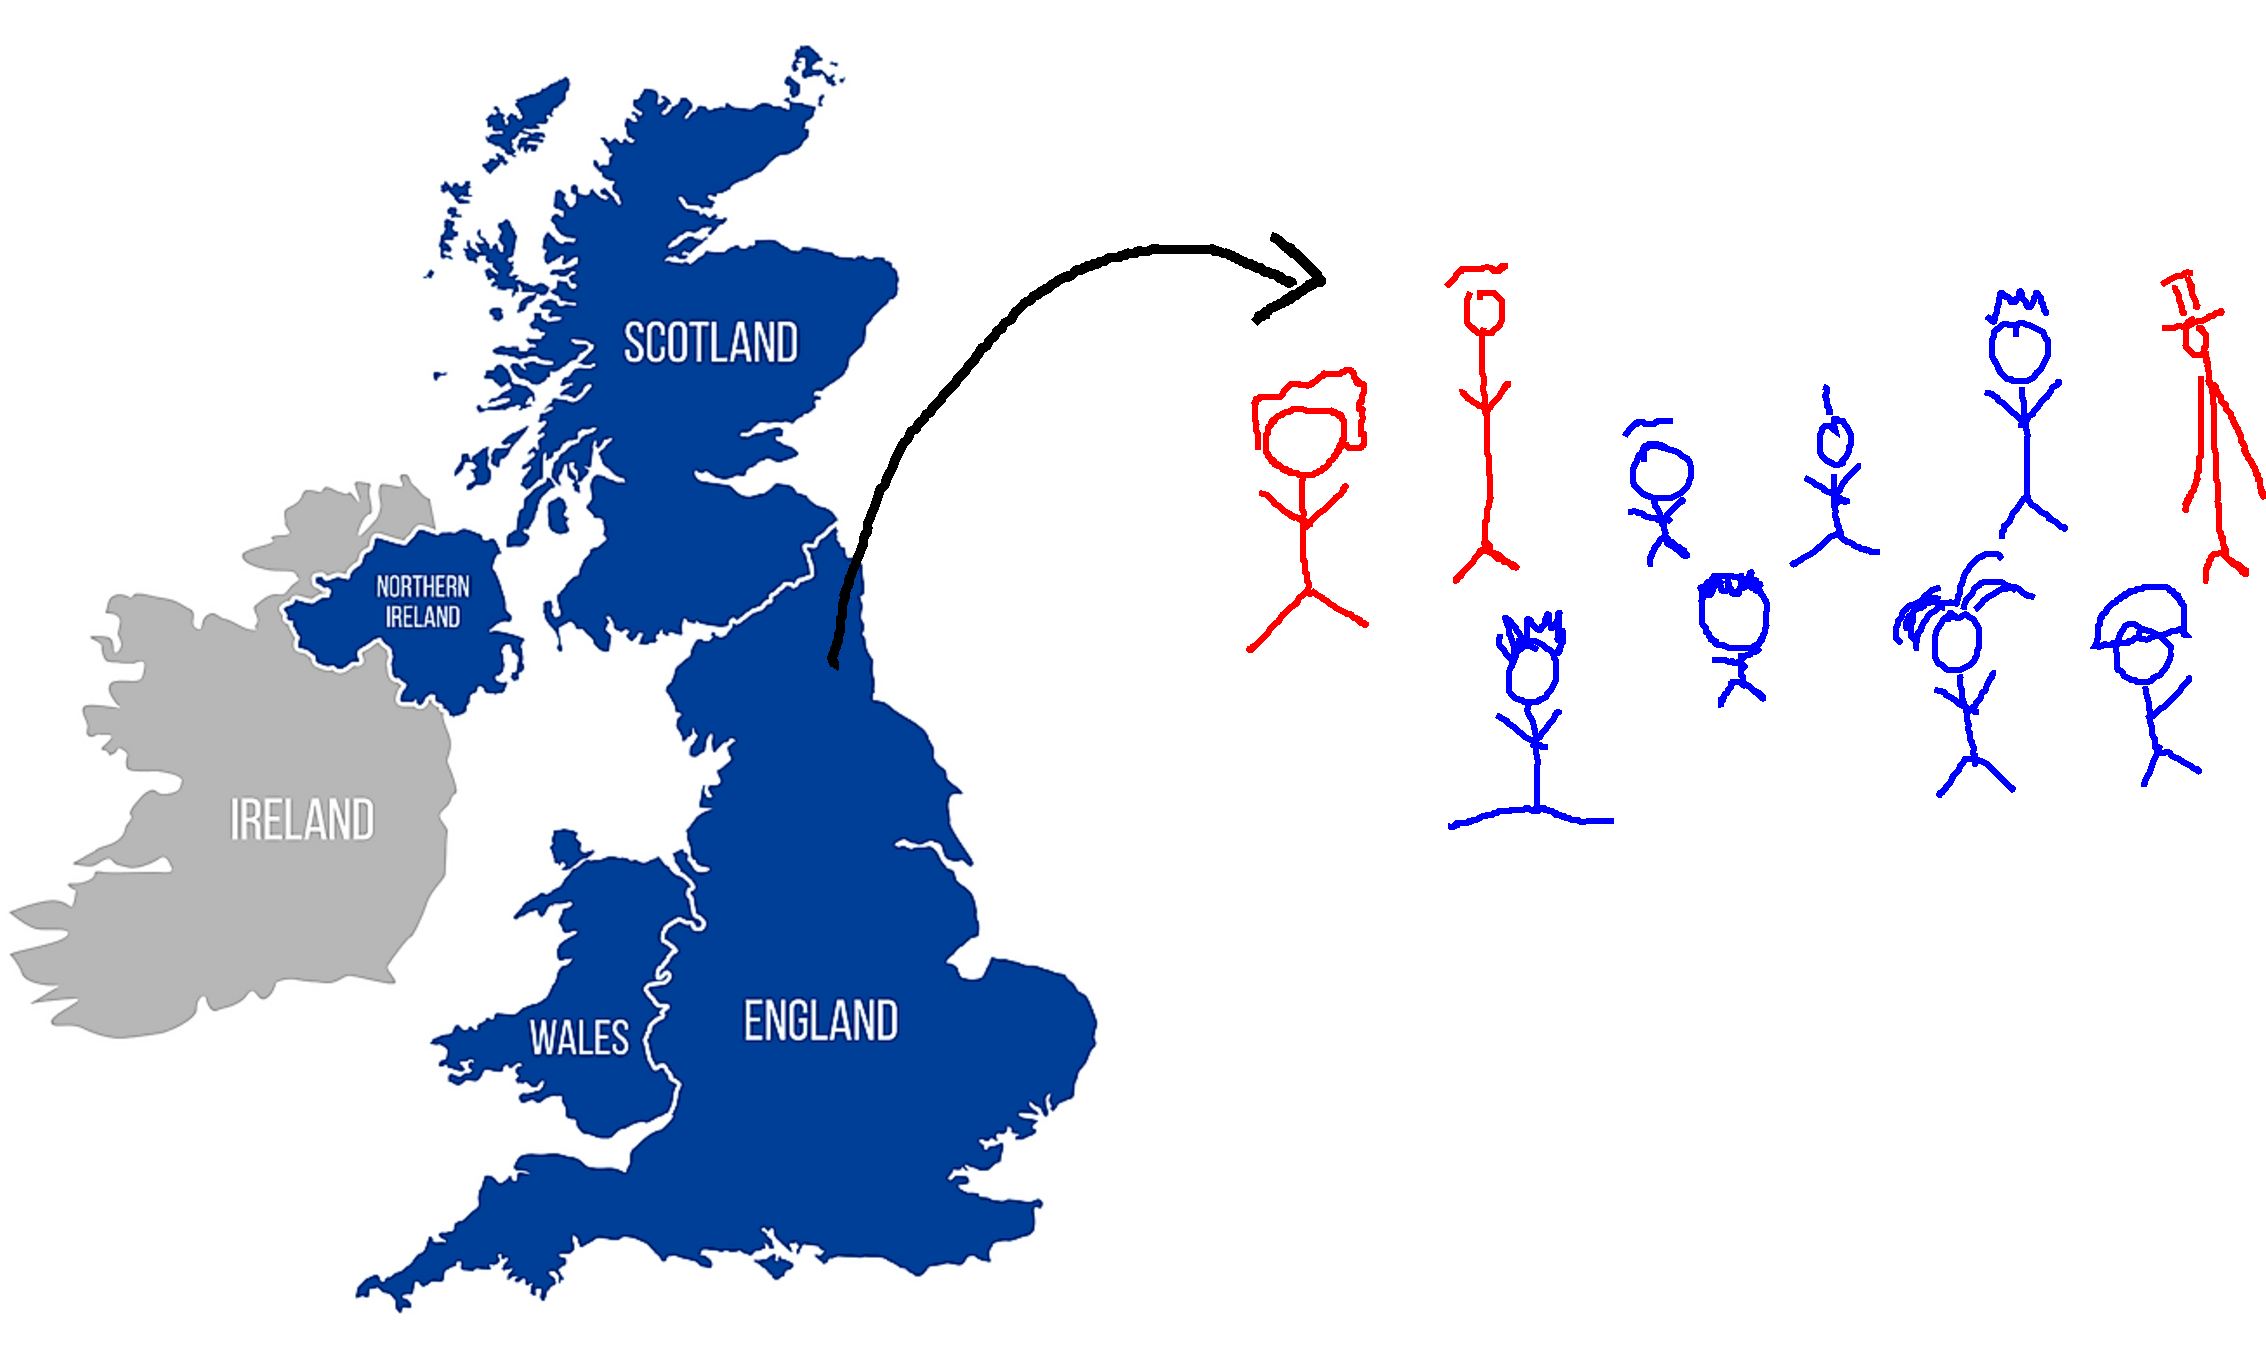
\includegraphics[width=1\textwidth]{./figures/uk-population.pdf}}
	\end{figure}
	
\end{frame}

\begin{frame}
	\frametitle{What probability model to use?}
	
	Again, we could use a \textit{binomial} model.
	
	\vspace{0.5cm}
	
	Note, very different problems often can share the same probability model.
	
\end{frame}

\begin{frame}
	
	\Large Questions?
\end{frame}

\section{Estimating interesting quantities}
\frame{\tableofcontents[currentsection]}


\section{Unpicking the signal from the noise}
\frame{\tableofcontents[currentsection]}


\begin{frame}
	\frametitle{That's it!}
	
	\Large Questions?
\end{frame}


\end{document}
